\documentclass[conference]{IEEEtran}
\IEEEoverridecommandlockouts
% The preceding line is only needed to identify funding in the first footnote. If that is unneeded, please comment it out.
\usepackage{cite}
\usepackage{amsmath,amssymb,amsfonts}
\usepackage{algorithmic}
\usepackage{graphicx}
\usepackage{textcomp}
\usepackage{xcolor}
\def\BibTeX{{\rm B\kern-.05em{\sc i\kern-.025em b}\kern-.08em
    T\kern-.1667em\lower.7ex\hbox{E}\kern-.125emX}}
    
    
\usepackage{caption}% <-- added
\captionsetup[table]{skip = 3pt}
\usepackage{tabulary}
\usepackage[para]{threeparttable}
\usepackage{array,booktabs,longtable,tabularx}
\newcolumntype{L}{>{\raggedright\arraybackslash}X}% <-- added
\usepackage{ltablex}% <-- added
\usepackage{siunitx}% <-- added
\usepackage{caption}% <-- added
\usepackage{pbox}% <-- added

\begin{document}

\title{Avaliação do desempenho de algoritmos de ML e IA associados a features de token e fuzzy}

\author{\IEEEauthorblockN{1\textsuperscript{st} Augusto Samuel Modesto}
\IEEEauthorblockA{\textit{Universidade de Brasília (UnB)} \\
Brasília, Brasil \\
augusto.modestoo@live.com}
\and
\IEEEauthorblockN{2\textsuperscript{nd} Marcus Fabricio Ferreira Paula}
\IEEEauthorblockA{\textit{Universidade de Brasília (UnB)} \\
Brasília, Brasil \\
marcus.fabricio@gmail.com}
}

\maketitle

\begin{abstract}
No passado, o acesso a informação era uma ideia distante da realidade da maior parte da população. Hoje, com o avanço tecnológico, em especial da internet, pessoas de qualquer parte do mundo podem se conectar instantaneamente. Com isso, comunidades e fóruns de perguntas e respostas se popularizou na internet. E a medida que o número de usuários aumenta, o número de dados e perguntas duplicadas também cresce. Nesse contexto, o objetivo desse trabalho é classificar se essas perguntas são duplicadas de modo automatizado. Para isso, apresenta-se uma avaliação de desempenho, por meio de uma abordagem, de algoritmos de machine learning e rede neural associados a combinação de modelos de dados diferentes, envolvendo features de token e fuzzy. Como resultado, aceitamos a hipótese de que as features e token e fuzzy em junção de algorítimos de regressão logística e XGBoost são melhores que utilizados de forma isolada e rejeitamos a hipótese de que a rede neural siamesa proposta desempenha melhor que a combinação dos modelos e algoritmos citados na hipótese anterior. 

\end{abstract}

\begin{IEEEkeywords}
nlp, similar questions, machine learning, classification, quora
\end{IEEEkeywords}

\section{Introdução}

Antes da Era Digital, as fontes de pesquisas disponíveis se limitavam, de forma física, a livros e enciclopédias ou, de forma tácita, por meio das aulas nas escolas, consultas com especialistas com algum grau de qualificação e do boca-a-boca de pessoas de uma comunidade. No início da década de 2000, os computadores se tornam peça chave na sociedade e, especialmente, com a popularização do computadores pessoas (PC) abriu-se uma gama de possibilidades de automatização de tarefas em escritórios e domésticas. Com esse avanço, a forma de como as pessoas buscavam conhecimento e a fonte de pesquisas dessas informações foram revolucionadas e constantemente sendo atualizadas.

O acesso a internet possibilitou a comunicação e o acesso rápido a qualquer parte do mundo de forma quase instantânea. Com isso, um fenômeno foi popularizado: o acesso as plataformas de perguntas e respostas, denominadas como comunidades de pergunta e resposta (do inglês: Community Question Answering - CQAs) \cite{Shah2009}. Dada a facilidade de participar e o acesso remoto a essas plataformas, foi possível fazer qualquer tipo de perguntas, bem como respondê-las.

Com a evolução dos buscadores de página web \cite{Ntoulas2004}, ficou cada mais fácil de encontrar as respostas para as perguntas desejadas. E com o tempo, um grande volume de dados e conhecimentos foram gerados e novos desafios tecnológicos começaram a surgir, dentre eles, o problema das perguntas duplicadas \cite{ravi2014}. 

As perguntas duplicadas se tornaram comuns a medida que o número de perguntas feitas nos CQAs aumenta. Isso representa um problema porque, quando tratadas de forma independentes, essas perguntas impedem que usuários vejam respostas de qualidade já existentes e que respondentes respondam a pergunta mais de uma vez \cite{sharma2019}.

Nesse contexto, a identificação bem sucedida de perguntas duplicadas reduz o tempo dos usuários na pesquisa de perguntas, facilita o acesso a respostas de qualidade já existentes e o reduz o esforço dos respondentes em termos de responder a versões distintas de uma mesma pergunta \cite{ravi2014, sharma2019}.

Com o avançado das técnicas de mineração de texto é possível mitigar esse esforço de identificar perguntas duplicadas e automatizar esse processo de classificação \cite{Zhang2015}.

Atualmente, a área de pesquisa de Processamento de Linguagem Natural (do inglês: Natural Language Processing, NLP) tem avançado em diversas soluções como: o método proposto em \cite{arora2015} que recuperam questões existentes e classificam como boas ou ruins em CQAs para inferir a qualidade de questões novas; a abordagem de classificação de clareza em perguntas realizadas em CQAs proposta por \cite{Trienes2019} baseada na noção de questões semelhantes; e a estrutura de aprendizado profundo de múltiplas instâncias proposto em \cite{Chen2017} que permite a predição da satisfação de User Interface (UI). Com base em como essas soluções foram concebidas, é possível automatizar a tarefa de classificação de perguntas duplicadas utilizando de mecanismos similares.

Nesse contexto, o objetivo dessa pesquisa é classificar se perguntas são duplicadas no contexto dos CQAs de modo automatizado. Para isso, foram criados modelos baseados em NLP. O treinamento desses modelos foram realizados no dataset da plataforma Quora. Quora é uma rede de perguntas e respostas onde os usuários fazem perguntas e outros usuários respondem.

As hipóteses levantadas para esta pesquisa são:
\begin{itemize}
\item (1) é possível ter melhores resultados incluindo à vetorização, recursos (features) de token e fuzzy dos pares de similaridade;

\item (2) redes neurais tem performance melhor que algoritmos lineares e árvores de decisão neste contexto.
\end{itemize}

As principais contribuições dessa pesquisa são:

\begin{itemize}
\item a associação de um conjunto de métricas de token e fuzzy aos vetores de palavras: isso ajuda os modelos a terem resultados melhores durante a fase de treinamento.
\item a constatação de que rede neural siamesa criada não é mais eficiente que modelos lineares e árvores de decisão no contexto proposto.
\end{itemize}

\section{Trabalhos relacionados}

A identificação de perguntas duplicadas faz parte de um ramo já conhecido em NLP, a correspondência de frase em linguagem natural (do inglês: Natural Language Sentence Matching - NLSM) cujo objetivo é determinar se duas frases são correspondentes ou não \cite{Wang2017}.

Segundo Sharma et. al. \cite{sharma2019}, para problemas como a identificação de perguntas duplicadas, é necessário que o modelo proposto seja capaz de identificar algumas características lexicais e sintáticos das perguntas, tais como tempo verbal, modalidade e ambiguidade sintática.

Os autores de \cite{sharma2019} testaram diferentes modelos de aprendizagem de máquina. Eles identificaram que a rede neural Continuous Bag of Words obteve bons resultados nos testes realizados. Contudo, os autores criaram uma base de teste própria para validação dos modelos utilizados no experimento.

Uma abordagem similar foi realizado por \cite{Byron2017}, onde os autores realizaram a extração de features de similaridade sintática e semântica das perguntas do banco de dados (dataset) proposto. Adicionalmente, foi utilizada a abordagem de aprendizagem pairwise-preference para realizar o ranqueado da ordem das perguntas e o treinamento com random florest para a classificação das perguntas. Nesta pesquisa realizada pelo autores, a ordem das questões é um fator importante porque faz parte da contextualização do problema, em que um dos objetivo é classificar as perguntas relevantes acima das irrelevantes dada uma perguntas candidata.

Inspirado no modelo de Manhatten LSTM \cite{Mueller2016}, os autores de \cite{Chen2017-2} propuseram uma nova arquitetura de memória de longo-curto prazo (do inglês: Long-Short Term Memory - LSTM) siamesa na qual utilizam duas sub-redes LSTM idênticas e classificam perguntas duplicadas a partir de uma rede neural de 3 camadas. 

Os autores em \cite{Chali2018}, também propõem uma abordagem voltada para redes recorrentes LSTM. Eles implementaram uma estrutura de modelos de arquitetura siamesa utilizando redes LSTM e memória bidirecional de longo-curto prazo (do inglês: Bi-direction Long-Short Term Memory - biLSTM) para a tarefa de identificação de perguntas duplicadas. Adicionalmente, foi inserido uma Rede Neural Convolucional (do inglês: Convolutional Neural Network - CNN) em junção as redes recorrentes como uma nova abordagem para a representação de sentenças.

A dificuldade de mapear automaticamente a semântica da linguagem natural em linguagens de programação é um problema abordado em \cite{Bhattacharjee2019}. Para solucionar o mesmo problema de identificação de perguntas duplicadas, os autores utilizam uma abordagem focada na ontologia, como o Web Ontology Language (OWL). As descobertas identificadas no trabalho mostram a viabilidade do uso de técnicas de PNL em conjunto com identificação de princípios de Linked Data.

No contexto da medicina, o problema de identificação de perguntas duplicadas em CQAs é recorrente, uma vez que pacientes anseiam por respostas as suas necessidades de saúde. No entanto, segundo \cite{McCreery2020}, os modelos comumente utilizados para resolver esse tipo de tarefa não generalizam bem para domínios de conhecimentos especializados, como o domínio médico. Para contornar esse problema, os autores propõem uma abordagem de duplo fine-tuning de uma rede neural pré-treinada em pares de perguntas e respostas.

\section{Dataset Quora de perguntas similares}

A plataforma Quora\footnote{https://pt.quora.com/} é um ambiente para compartilhamento de conhecimento sobre diversos assuntos. Seus usuários podem fazer perguntas e conectar-se com diferentes pessoas para contribuir com suas perspectivas exclusivas acerca de diversos tipos de perguntas. A plataforma tem em média 100 milhões visitantes a cada mês, contando com um amplo volume dados de texto. 

A Quora Question Pairs é uma competição Kaggle\footnote{https://www.kaggle.com/c/quora-question-pairs} inativa, que desafia os participantes a lidar com o problema de NLP de classificação de perguntas duplicadas. A organização da competição disponibiliza de forma gratuita o dataset\footnote{https://www.kaggle.com/c/quora-question-pairs/data}.

O dataset é composto por um conjunto de treinamento de 404.290 pares de perguntas e um conjunto de teste de 2.345.795 pares de perguntas. Não há disponibilização de um conjunto de validação. Todos os pares de perguntas são escrito na língua inglesa.

Na Tabela 1, são fornecidos alguns exemplos de como os pares de perguntas formam o dataset.

\begin{table}[]
\captionsetup{}
\caption{Exemplos de observações do dataset original.} \label{tab:freq}
\setlength\tabcolsep{0pt} % let LaTeX compute intercolumn whitespace
\footnotesize\centering

\smallskip 
\begin{tabular*}{\columnwidth}{@{\extracolsep{\fill}}rccccc}
\toprule
  id & qid1 & qid2 & question1 & question2 & isduplicate \\
\midrule
  0 & 1 & 2 &
   \pbox{10cm}{What is the step \\ by step guide to \\ invest in share market \\ in india?\\} &
  \pbox{10cm}{What is the step \\ by step guide to \\ invest in share market?\\} &
  0 \\
  
  5 & 11 & 12 &
  \pbox{10cm}{Astrology: I am a \\ Capricor Sun Cap \\ moon and cap rising... \\ what does that say \\ about me?\\} &
  \pbox{10cm}{I'm a triple Capricorn \\ (Sun, Moon and \\ ascendant in Capricorn) \\ What does this say \\ about me?\\} &
  1 \\ \hline
\bottomrule
\end{tabular*}
\end{table}

Os campos presentes neste dataset são:
\begin{itemize}
\item id: ID único de cada par;
\item qid1: ID da primeira pergunta;
\item qid2: ID da segunda pergunta;
\item question1: texto da primeira pergunta;
\item question2: texto da segunda questão;
\item is\_duplicate: se as perguntas 1 e 2 são duplicadas o valor é 1. O valor é 0 caso contrário. 
\end{itemize}


O conjunto de teste fornecido pela competição não possui rótulos. Isso implica que não é possível medir outras métricas que não sejam as utilizadas na competição, uma vez que é necessário submeter os resultados da inferência do conjunto de teste à plataforma. A métrica de avaliação utilizada na competição é o log loss.

Para mitigar esse impedimento, foi criado um conjunto de testes a partir do conjunto de treinamento. Isso permitirá a aferição de novas métricas além da log loss, obrigatória na competição.

Diferentemente da pesquisa realizada por \cite{McCreery2020} que construíram um dataset de pares de perguntas especializada para o contexto médico, o dataset utilizado nessa pesquisa é genérico e contém um grande corpus de pares de perguntas. As informações sobre a divisão do dataset são exploradas na subseção 4.A.

\section{Visão geral da abordagem}

Em resumo, o objetivo dessa pesquisa é classificar se perguntas são duplicadas ou não em um contexto de CQA. Para atender a esse objetivo, é proposto a construção de seis modelos de dados combinando a criação de features com algoritmos de aprendizagem de máquina (do inglês: Machine Learning - ML) e rede neural.

Para atender ao objetivo proposto, uma abordagem foi criada e executada. A partir dessa abordagem, inicialmente, o dataset foi reamostrada e as proporções de cada classe foram reajustadas. Um conjunto de dados de treino e teste foi remanejado a partir dessa reamostragem. Os detalhes são abordados na subseção 4.A.

O pré-processamento dos dados consistiu em realizar a limpeza da base, como remoção de pontuação e stop words, conversão de dados dispensáveis e descontração de palavras inglesas. Os detalhes são abordados na subseção 4.B.

Foi executado um processo de engenharia de recursos (Featurização) e a vetorização dos recursos textuais. Os detalhes são abordados na subseção 4.C.

Foram construídos cinco modelos para realizar a classificação combinados com a utilização dos algoritmos de ML como a regressão logística (do inglês: Logistic Regression - LR) e o XGBoost. E um 6º modelo foi construído combinado com uma rede neural Siamesa. Os detalhes são abordados na subseção 4.D.

Os modelos foram avaliados com base nas métricas: acurácia, F1-score e log loss.
Os detalhes são abordados na subseção 4.E.

Um resumo da visão geral da abordagem adotada nessa pesquisa pode ser visualizada na Figura 1.

\begin{figure*}[htbp]
  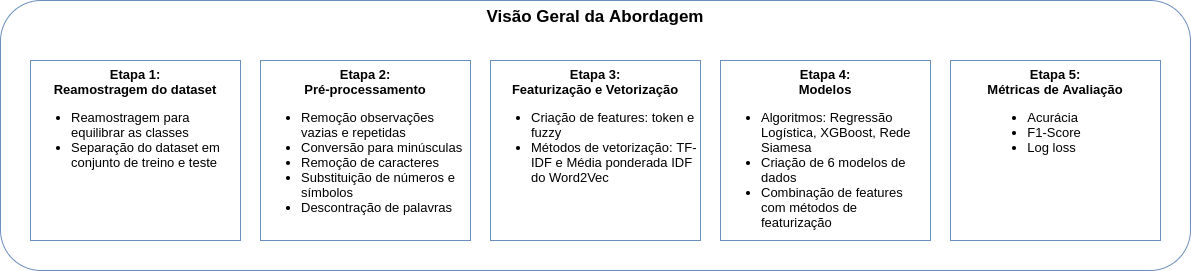
\includegraphics[width=\textwidth]{abordagem.png}
  \caption{Visão Geral da Abordagem da Pesquisa.}
\end{figure*}

\subsection{Reamostragem do dataset}

Originalmente o dataset de treino apresenta 404.290 pares de perguntas. Dentre os pares, há três pares com perguntas nulas. Elas foram removidas, resultando em um total de 404.287 observações. Esse dataset tem a proporção de 63\% de pares não-similares e 37\% de pares similares. O dataset de teste original não possuí rótulos.

O dataset de treino foi reduzido para que as classes pudessem ser balanceadas e para que os treinamentos dos modelos pudessem ser realizados com menos tempo e consumo de recursos. Essa redução foi sistematizada em dois passos: (1) reamostragem para equilibrar as classes (similar e não-similar); (2) separação do dataset em conjunto de treino e teste.

Para realizar o passo (1), o conjunto de treino foi reamostrado em dois subconjuntos de dados com pares similares e não similares. De cada subconjunto, 149.263 pares de perguntas foram aleatoriamente sorteados e selecionados. Os pares restantes foram descartados. Os subconjuntos selecionados foram unificados e as amostras foram embaralhados para manter a aleatoriedade da ordem dos pares.

Ao final da reamostragem, o novo conjunto de treino possuía 298.526 observações. E cada classe ficou representada por 50\% das amostras.

Para realizar o passo (2), uma amostra de teste foi extraída do conjunto de treino. A proporção da extração corresponde a 30\% do conjunto de treino. Essa técnica é denominada como Hold-Out Validation e é comumente utilizada na comunidade de ciência de dados assumindo uma proporção entre 10\% a 30\% de acordo com o contexto dos dados \cite{Yadav2016}. O conjunto de teste manteve a proporção original das classes de 50\% de pares não-similares e 50\% de pares similares.

Ao final da divisão dos conjuntos de treino e teste, os conjuntos ficaram com 208.968 e 89.558 amostras respectivamente.

\subsection{Pré-Processamento}

A fase de pré-processamento é importante no contexto da NLP porque reduz o tamanho do vocabulário. Essa redução tem impacto significativo durante a fase de treinamento dos modelos, uma vez que o tempo e o consumo de recursos são reduzidos também. Além disso, essa fase pode ser realizada de diferentes maneiras de acordo com o estado atual do dataset utilizado.

No contexto do dataset dessa pesquisa, a primeira tarefa de pré-processamento realizada foi a limpeza de observações vazias. Ela foi realizada durante a amostragem do dataset, conforme apresentado na subseção 4.A.

A segunda tarefa foi verificar a presença de observações repetidas. Para isso, os campos de identificação única (id, qid1 e qid2) foram avaliados para identificar a ocorrência de duplicidade. Nenhum registro duplicado foi encontrado.

A terceira etapa foi a conversão de todos os pares de perguntas em minúsculas. Isso possibilita que as etapas de pré-processamento posteriores sejam executadas mais facilmente.

A quarta etapa foi a execução de um script python para remoção de caracteres inválidos ou dispensáveis para o processo de vetorização. O script removeu:
pontuações; tags HTML como $<html>$ e $<title>$; e stop words, que são palavras que não fornecem significado semântico, como 'this', 'it' e 'each'.

A quinta etapa foi a execução de um script python para substituição de: valores números por strings, como por exemplo 1.000.000 com 1m; e caracteres especiais por seus equivalentes em string, por exemplo \$ por 'dollar', \% por 'percent' e etc.

E a sexta e última etapa foi a descontrações das palavras. Essa requisito é especialmente importante em um vocabulário inglês. Para realizar essa atividade, foi utilizada a página da wikipedia\footnote{List of English contractions from Wikipedia:

https://en.wikipedia.org/wiki/Wikipedia\%3aList\_of\_English\_contractions} que listas todas as contrações recorrentes no inglês.

Após aplicação de todas as etapas, pode-se visualizar, na Tabela 2, o resultado da aplicação do pré-processamento nos mesmos exemplos da Tabela 1.

\begin{table}[]
\captionsetup{}
\caption{Exemplos de observações após o pré-processamento.} \label{tab:freq}
\setlength\tabcolsep{0pt} % let LaTeX compute intercolumn whitespace
\footnotesize\centering

\smallskip 
\begin{tabular*}{\columnwidth}{@{\extracolsep{\fill}}rccccc}
\toprule
  Pergunta 1 & Pergunta 2 & Duplicado \\
\midrule
  \pbox{3cm}{step step guide invest share market india \\} &
  \pbox{3cm}{step step guide invest share market \\} &
  \pbox{3cm}{0\\} \\
  
  \pbox{3cm}{astrology capricor sun cap moon cap rising say \\} &
  \pbox{3cm}{triple capricorn sun moon ascendant capricorn say \\} &
  \pbox{3cm}{1\\} \\ \hline
\bottomrule
\end{tabular*}
\end{table}


Não foi executado nenhum processo de lematização (stemming ou lemmatization) porque consume um tempo de execução consideravelmente grande para a quantidade de palavras presentes no dataset. Além disso, é comum haver nas perguntas presente no dataset trocadilhos intencionais que seriam prejudicados durante o processo de lematização.

\subsection{Engenharia de Features e Vetorização}

A engenharia de features (ou featurização) é um dos processos mais importantes para o treinamento de NLP, pois é por meio dos resultados dessa etapa que os algoritmos de ML são alimentados \cite{Aroyehun2018}.

A hipótese (1) apresentada nessa pesquisa consiste na afirmativa de que é possível ter resultados melhores incluindo à vetorização, features de token e fuzzy dos pares de similaridade. Com base nisso, foram criadas algumas features para testar essa hipótese.

O primeiro conjunto de features criado foi o de tokens, que são extraídos a partir das palavras (tokens) das duplas de perguntas similares do dataset. Esse tipo de feature é comumente utilizado em tarefas de NLP.

As features de tokens criadas foram divididas em quatro categorias: contadoras; proporções; condicionais; e comprimento dos tokens.

As features de tokens contadoras que foram definidas são:
\begin{itemize}
\item words\_question1 e words\_question2: número de palavras na questão 1 e 2;
\item len\_question1 e len\_question2: número de caracteres na pergunta 1 e 2;
\item mutual\_words: Número de palavras que ocorrem na pergunta 1 e na 2. Quando as palavras são repetidas, elas não são contabilizadas;
\item count\_mutual\_adjective: é o número de adjetivos comuns em ambas as perguntas;
\item count\_mutual\_proper\_name: é o número de nomes próprios comuns em ambas as perguntas;
 \item count\_mutual\_noun: é o número de substantivos comuns em ambas as perguntas;
\end{itemize}

As features de tokens de proporções são:
\begin{itemize}
\item ratio\_min\_stop\_words\_question: é a proporção entre o número de stop words comuns e o comprimento da menor pergunta.
\item ratio\_max\_stop\_words\_question: é a proporção entre o número de stop words comuns e o comprimento da maior pergunta.
\item ratio\_min\_token\_words: é a proporção do número de token comuns para o menor token entre as duas perguntas.
\item ratio\_max\_token\_words: é a proporção do número de token comuns para o maior token entre as duas perguntas.
\end{itemize}

As features de tokens condicionais são:
\begin{itemize}
\item first\_token\_equals: é 0 se nas perguntas o primeiro token não é o mesmo, e 1 caso seja o mesmo token.
\item last\_token\_equals: é 0 se nas perguntas o último token não é o mesmo, e 1 caso seja o mesmo token.
\end{itemize}

As features de comprimento dos tokens são:
\begin{itemize}
\item len\_mean: é a média do comprimento (número de tokens) de ambas as perguntas.
\item len\_median: é a mediana do comprimento de ambas as perguntas.
\item ratio\_max\_min: é a razão entre o comprimento da maior perguntas e o comprimento da menor perguntas.
\item absolute\_difference: é a diferença absoluta entre o comprimento de ambas as perguntas.
\end{itemize}

O último conjunto de features criado foi o de fuzzy, que são extraídos a partir da comparação da equivalência de strings das duplas de perguntas similares.

As features de fuzzy foram criadas a partir do pacote FuzzyWuzzy do python. O pacote utiliza a distância de Levenshtein \cite{Lev1966} para comparar as strings. Essa biblioteca é útil uma vez que fornece recursos simples, porém robustos de comparar similaridade entre strings, ideal para o contexto desta pesquisa.

As features fuzzy selecionadas foram:
\begin{itemize}
\item ratio\_parcial\_fuzz: corresponde ao método fuzz.partial\_ratio(), que identifica correspondências de strings mais complexas que as utilizadas no método fuzz.ratio();
\item ratio\_sorte\_token: corresponde ao método fuzz.token\_sort\_ratio(), que permite classificar uma sequência de tokens em ordem alfabética. Isso é útil quando os tokens comparados têm a mesma grafia, mas não estão na mesma ordem;
\item ratio\_set\_token: corresponde ao método fuzz.token\_set\_ratio(), que
considera os tokens comuns durante a comparação de strings. Isso é útil quando aplicada a um conjunto de tokens que tem uma diferença de comprimento da string.
\end{itemize}

Quanto ao processo de vetorização, que consiste em capturar o significado semântico de frases por meio de vetores \cite{Beng2018}, foram definidos dois métodos: o Term Frequency Inverse Document Frequency (TF-IDF), e a média ponderada IDF do Word2Vec. 

O TF-IDF é a razão entre o número de vezes que uma palavra $t$ ocorre no documento $d$ dividido pelo número total de palavras no documento $d$. Em suma, quanto maior o valor TF-IDF, mais alto é a probabilidade de encontrar a palavra $t$ no documento $d$, e isso indica que $t$ é uma palavra importante no corpus específico \cite{Salton1988}.

O Word2Vec captura informações contextuais de uma dada palavra por meio de um espaço vetorial, de tal forma que a localização dessa palavra é determinada pelo seu significado. Ou seja, palavras com significados semelhantes tem maior proximidade, no espaço vetorial, que palavras com significados diferentes ou opostos.

\begin{figure*}[htbp]
  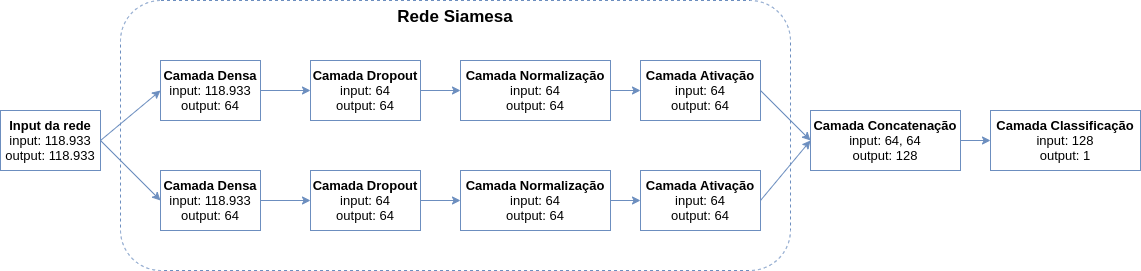
\includegraphics[width=\textwidth]{rede_siamesa.png}
  \caption{Arquitetura da Rede Siamesa.}
\end{figure*}

Um benefício da utilização do Word2Vec é que é possível calcular a distância do cosseno, valor do cosseno do ângulo entre dois vetores, para determinar a similaridade de palavras.

Para calcular a média ponderada IDF do Word2Vec é necessário multiplicar o vetor de cada palavra por seu valor IDF obtendo os vetores ponderados IDF, adicionar todos os vetores ponderados IDF em uma frase, e dividir pelo número de palavras na frase \cite{Dja2019}.

Com a execução de ambos os métodos, as dimensões do dataset resultantes foram:
\begin{itemize}
    \item Vetorização com o TF-IDF: 59.457 dimensões por pergunta. Totalizando 118.914 dimensões ao somar as perguntas 1 e 2.
    \item Vetorização com a média ponderada IDF do Word2Vec: 300 dimensões por pergunta. Totalizando 600 dimensões ao somar as perguntas 1 e 2.
\end{itemize}

\subsection{Modelos}

Para resolver o problema explanado nessa pesquisa, identificar perguntas duplicadas, será realizada a tarefa de classificação utilizando algoritmos de ML e rede neural. 

Foi escolhido um algoritmo das classes de modelos de regressões, de árvores de decisão e de redes neurais artificias, sendo a Regressão Logística, o XGBoost e a rede Siamesa as escolhas das respectivas classes.

Quanto aos modelos de dados, eles consistem na combinação dos resultados dos processos de vetorização e featurização realizados anteriormente. O objetivo de testar mais de um modelo tem como intuito validar a hipótese (1) definida.

Para esta pesquisa, foram criados seis modelos distintos. As combinações definidas para cada um deles são apresentados na Tabela 3. O campo \textit{Características} define a combinação que será utilizada no treinamento do modelo.

\begin{table}[]
\captionsetup{}
\caption{Modelos de dados definidos para pesquisa.} \label{tab:freq}
\setlength\tabcolsep{0pt} 
\footnotesize\centering
\smallskip 
\begin{tabular*}{\columnwidth}{@{\extracolsep{\fill}}rccccc}
\toprule
  Nº Modelo & Características & Algoritmo & Dimensões \\
\midrule
    Modelo 1 & \pbox{3cm}{ $ $ \\Features (token e fuzzy) \\} & LR e XGBoost & 21 \\ 
    Modelo 2 & \pbox{3cm}{ $ $ \\ TF-IDF \\} & LR e XGBoost &  118.914 \\ 
    Modelo 3 & \pbox{3cm}{ $ $ \\ Média ponderada IDF do Word2Vec \\} & LR e XGBoost & 600 \\ 
    Modelo 4 & \pbox{3cm}{TF-IDF + Features} & LR e XGBoost & 118.935 \\ 
    Modelo 5 & \pbox{3cm}{ $ $ \\ Média ponderada IDF do Word2Vec + Features \\} & LR e XGBoost & 621 \\ 
    Modelo 6 & TF-IDF & Rede Siamesa & 118.914 \\ 
\hline
\bottomrule
\end{tabular*}
\end{table}

Para o modelo LR, foi escolhido um único conjunto de hiperparâmetros para ser utilizado em todos os modelos. Eles são: alfa = 0.00001; e a penalidade escolhida foi a regularização ElasticNet.

Para o modelo XGBoost, também foi escolhido um único conjunto de hiperparâmetros para ser utilizado em todos os modelos. Eles são: estimadores = 100; e profundidade = 6.

Para a rede Siamesa, os hiperparâmetros definidos foram: batchz\_size = 64; epochs = 20; optimizers = Adam; e learning\_rate = 0.01.

O uso de rede Siamesas para detecção de similaridade semântica textual não é novidade na área de NLP. Autores como \cite{Neculoiu2016} e \cite{Ranasinghe2019} já exploração o uso desse recurso. Para essa pesquisa, foi duplicada a rede Siamesa utilizada em \cite{Ritvik2021} e ajustado os hiperparâmetros de conforme o objetivo proposto.

Essa arquitetura de rede Siamesa é simples e conta com uma camada densa de 118.933 parâmetros, seguido de uma camada dropout, uma normalização e uma ativação. Posteriormente os resultados das subredes siamesas são concatenados e classificados. Na Figura 2 é apresentada a arquitetura da rede siamesa implementada para essa pesquisa.


\subsection{Métricas de avaliação dos modelos}

As métricas para avaliação dos modelos definidos para essa pesquisa foram a acurácia, o F1-score e o log loss. Essas métricas foram baseadas na abordagem adotada em \cite{sharma2019}.

O objetivo da adoção da acurácia foi avaliar a performance geral do modelo. Essa métrica permite avaliar dentre todas as classificações, quantas o modelo classificou corretamente. 

Quanto ao F1-score, seu objetivo foi em avaliar a geração de falsos positivos e falsos negativos. Essa métrica compõe uma média harmônica entre as métricas de precisão (para avaliação de falsos positivos) e de recall (para avaliação de falsos negativos). Quando o um F1-Score é baixo, há um indicativo de que a precisão ou o recall está baixo.

E a log loss é uma métrica mais suave de acurácia, ao qual é incorporado a confiança probabilística dos resultados do modelo. O objetivo dessa métrica é punir erros grosseiros do modelo. Ela foi adotada porque também foi utilizada na competição do Kaggle para avaliar os resultados dos modelos produzidos.

\section{Resultados e Discussões}

Os resultados obtidos apontam que o modelo 5, executado com o algoritmo LR, tem maior precisão na inferência do conjunto de testes. Na Tabela 4 são apresentados os resultados dos modelos 1 a 5 com os algoritmos LR e XGBoost.

\begin{table*}
\captionsetup{}
\caption{Resultados das métricas para o conjunto de teste do LR e XGBoost.} \label{tab:freq}
\setlength\tabcolsep{0pt} 
\footnotesize\centering
\centering
\begin{tabular*}{\textwidth}{@{\extracolsep{\stretch{1}}}*{7}{r}@{}}
  \toprule
   & \multicolumn{3}{c}{{\textbf{Regressão Logística}}}  &  \multicolumn{3}{c}{{\textbf{XGBoost}}} \\
   \cmidrule(lr){2-4}\cmidrule(l){5-7}
   & \textbf{Log Loss} & \textbf{Acurácia} & \textbf{F1-Score} & \textbf{Log Loss} & \textbf{Acurácia} & \textbf{F1-Score} \\
  \midrule
    Modelo 1 & 0.55102 & 0.70486 & 0.71552 & 0.47443 & 0.76173 & 0.77820 \\ 
    Modelo 2 & 0.55030 & 0.71894 & 0.70863 & 0.58359 & 0.67565 & 0.60519 \\
    Modelo 3 & 0.65252 & 0.63148 & 0.63937 & 0.62977 & 0.68330 & 0.69850 \\
    Modelo 4 & 0.51556 & 0.74690 & 0.75843 & 0.49101 & 0.75968 & 0.78961 \\
    Modelo 5 & \textbf{0.43078} & \textbf{0.79773} & \textbf{0.80273} & \textbf{0.44134} & \textbf{0.78143} & \textbf{0.79544} \\
  \hline       
  \bottomrule
\end{tabular*}
\end{table*}


O modelo 5, que utiliza a média ponderada IDF do Word2Vec combinado com as features de token e fuzzy, teve desempenho superior nas três métricas definidas em relação as demais modelos. Esse resultado foi consistente tanto na regressão logística quanto no XGBoost. No entanto, a LR foi ainda melhor que o XGBoost, obtendo um log loss de 0.43078, acurácia de 0.79773, F1-Score de 0.80273. 

Apesar do resultado obtido pelo modelo 5 com LR ser melhor que os demais, 80\% de acurácia e F1-Score é um valor intermediário para a tarefa de classificação nesse contexto. Incrementar as features com novos indicadores como, por exemplo, a distância do cosseno (apenas com Word2Vec) ou utilizar métodos de vetorização mais robustos e eficaz como o BERT \cite{BERT2019} e o RoBERTa \cite{RoBERTa2019} podem ser alternativas para aumentar as métricas avaliadas.

Contudo, pode-se considerar a hipótese (1), dado o contexto da avaliação realizada, como aceita uma vez que foram obtidos resultados melhores com a inserção das features (token e fuzzy) nos modelos 4 e 5 para o algoritmo LR.
No entanto, para com o algoritmo XGBoost, o modelo 1 obteve resultado superior ao modelo 4 e inferior ao modelo 5. Dado que variação obtida é pequena, ajustes nos hiperparâmetros do XGBoost podem melhor os resultados obtidos ao custo de tempo de execução do algoritmo e de recursos computacionais para o processamento.

Quanto a rede Siamesa, executado no modelo 6, o resultado obtido foi superior no modelo 4 para o XGBoost, porém inferior ao modelo 4 para a LR e modelo 5 para ambos algoritmos. Na Tabela 5 é apresentado o resultado do modelo 6.

\begin{table}[]
\captionsetup{}
\caption{Resultado das métricas para o conjunto de teste da Rede Siamesa.} \label{tab:freq}
\setlength\tabcolsep{0pt} 
\footnotesize\centering
\smallskip 
\begin{tabular*}{\columnwidth}{@{\extracolsep{\fill}}rccc}
\toprule
  & \multicolumn{3}{c}{{\textbf{Rede Siamesa}}} \\
  \cmidrule(lr){2-4} \\
  & \textbf{Log Loss} & \textbf{Acurácia} & \textbf{F1-Score} \\
\midrule
    Modelo 6 & 0.67036 & 0.75417 & 0.76461 \\ 
\hline 
\bottomrule

\end{tabular*}
\end{table}

A rede Siamesa não teve um bom desempenho. Os hiperparâmetros definidos para esse modelo certamente tiveram um impacto nos resultados finais. Com um número de épocas (epochs) maior e uma taxa de aprendizagem (learning\_rate) menor, os resultados obtidos podem melhorar consideravelmente. No entanto, o custo disso é convertido no tempo de execução e consumo de recursos computacionais para o processamento, como já mencionado para outros algoritmos.

Outra solução plausível para esse contexto é a utilização de uma arquitetura de redes siamesas com LSTM, conforme abordados por \cite{Chen2017-2} e \cite{Chali2018}. Pois, elas tem uma capacidade de avaliação semântica melhor que a rede siamesa comum.

Com base nos dados obtidos neste contexto, a hipótese (2) foi rejeitada, uma vez que os resultados dos modelos 4 e 5 foram superiores ao modelo 6.

\section{Conclusões e Trabalhos futuros}
 
Nessa pesquisa, foi realizada uma reamostragem dos dados e o balanceamento das classes que compreendem o problema de classificação proposto (similar e não-similar). Posteriormente, foi executada uma limpeza nos dados, removendo observações vazias, stop words e tags html, convertendo dados dispensáveis para o entendimento semântico e descontração das palavras inglesas. Também foram executados os processos de featurização e vetorização com métodos diferentes. Isso possibilitou a construção de diferentes modelos de dados com base nas combinações dos resultados dessas técnicas. Com os resultados obtidos pelos modelos, viu-se que o regressão logística utilizando a média ponderada IDF do Word2Vec combinado com as Features de token e fuzzy tem um desempenho superior ao demais modelos avaliados. Além disso, os resultados possibilitaram o aceite da hipótese (1) e a rejeição da hipótese (2).

No futuro, os modelos propostos podem ser avaliados com técnicas de vetorização mais recentes e robustas como o BERT e o RoBERTa. A adição de mais features também é um passo que podem melhorar o desempenho dos modelos. Além disso, propõe-se que seja utilizados modelos de arquitetura de redes siamesas com LSTM e com uma parametrização mais aprimorada. Também propomos que seja realizado a tradução do dataset do inglês para o português para avaliar se o desempenho da classificação é melhorada.

\begin{thebibliography}{00}

\bibitem{Shah2009} C. Shah, S. Oh, and J. S. Oh. Research agenda for social Q\&A, Library \& Information Science Research. Volume 31, Issue 4, pp. 205-209, ISSN 0740-8188, 2009 https://doi.org/10.1016/j.lisr.2009.07.006.

\bibitem{Ntoulas2004} A. Ntoulas, J. Cho, and C. Olston. What's new on the web? the evolution of the web from a search engine perspective. In Proceedings of the 13th international conference on World Wide Web (WWW '04). Association for Computing Machinery, New York, NY, USA, pp. 1–12, 2004. DOI:https://doi.org/10.1145/988672.988674

\bibitem{ravi2014} S. Ravi, B. Pang, et al. Great Question! Question Quality in Community Q\&A. ICWSM, v. 14, pp. 426-435, 2014.

\bibitem{sharma2019} L. Sharma et al. Natural Language Understanding with the Quora Question Pairs Dataset. In ArXiv abs/1907.01041. 2019.

\bibitem{Zhang2015} Zhang, Y., et al. Multi-Factor Duplicate Question Detection in Stack Overflow. J. Comput. Sci. Technol. 30, 981–997, 2015. https://doi.org/10.1007/s11390-015-1576-4

\bibitem{arora2015} P. Arora, Ganguly, D., and Jones, G. J. F. The Good, the Bad and their Kins: Identifying Questions with Negative Scores in StackOverflow. Proceedings of the 2015 IEEE/ACM International Conference on Advances in Social Networks Analysis and Mining 2015. Paris, France: ACM: pp. 1232-1239, 2015.

\bibitem{Trienes2019} Jan Trienes, and Krisztian Balog. Identifying Unclear Questions in Commu-nity Question Answering Websites. In Springer International Publishing: Advances in Information Retrieval. pp. 276–289, 2019.

\bibitem{Chen2017} Chen, Z., et. al. User personal-ized satisfaction prediction via multiple instance deep learning. InInternationalConference on World Wide Web (WWW). pp. 907–915, 2017.

\bibitem{Wang2017} Zhiguo Wang, Wael Hamza, and Radu Florian. Bilateral multi-perspective matching for natural language sentences. In Proceedings of the 26th International Joint Conference on Artificial Intelligence (IJCAI'17). AAAI Press, pp. 4144–4150, 2017.

\bibitem{Byron2017} Byron V. Galbraith and Bhanu Pratap and D. Shank. Talla at SemEval-2017 Task 3: Identifying Similar Questions Through Paraphrase Detection. In Proceedings of the 11th International Workshop on Semantic Evaluations (SemEval-2017), pp. 375–379, Vancouver, Canada, August 3 - 4, 2017.

\bibitem{Mueller2016} J. Mueller and A. Thyagarajan. Siamese Recurrent Architectures for Learning Sentence Similarity. In Proceedings of the Thirtieth Conference on Artificial Intelligence, Phoenix, Arizona, USA, pp. 2786–2792, 2016. 

\bibitem{Chen2017-2} Zihan Chen, et. al. Quora Question Pairs. 2017. Available: http://static.hongbozhang.me/doc/STAT\_441\_Report.pdf

\bibitem{Chali2018} Yllias Chali, and Rafat Islam. Question-Question Similarity in Online Forums. In Proceedings of the 10th annual meeting of the Forum for Information Retrieval Evaluation (FIRE'18). Association for Computing Machinery, New York, NY, USA, pp. 21–28, 2018. DOI:https://doi.org/10.1145/3293339.3293345


\bibitem{Bhattacharjee2019} Anirban Bhattacharjee. Identifying Semantically Similar questions using NLP techniques and Linked Data Principles. M.S. thesis, University of Dublin, Trinity College. August, 2019. Available: http://fabriziorlandi.net/pdf/2019/Anirban\_2019\_MSc\_Dissertation.pdf

\bibitem{McCreery2020} Clara H. McCreery, et. al. Effective Transfer Learning for Identifying Similar Questions: Matching User Questions to COVID-19 FAQs. Proceedings of the 26th ACM SIGKDD International Conference on Knowledge Discovery \& Data Mining. Association for Computing Machinery, New York, NY, USA, pp. 3458–3465, 2020 DOI:https://doi.org/10.1145/3394486.3412861

\bibitem{Yadav2016} S. Yadav and S. Shukla. Analysis of k-Fold Cross-Validation over Hold-Out Validation on Colossal Datasets for Quality Classification. 2016 IEEE 6th International Conference on Advanced Computing (IACC), pp. 78-83, 2016, doi: 10.1109/IACC.2016.25. 

\bibitem{Aroyehun2018} Aroyehun, Segun and Angel, Jason and Alvarez, Daniel and Gelbukh, Alexander. Complex Word Identification: Convolutional Neural Network vs. Feature Engineering. pp. 322-327. 10.18653, v1, W18-0538, 2018. 

\bibitem{Lev1966} V. Levenshtein. “Binary codes capable of correcting deletions, insertions, and reversals” Soviet Physics Doklady, vol.10, no.8, pp. 707­710, 1966.

\bibitem{Beng2018} B. Bengfort, R. Bilbro, and T. Ojeda, Applied Text Analysis with Python: Enabling Language-Aware Data Products with Machine Learning, 1st ed.
O’Reilly Media Incorporated, 2018.

\bibitem{Salton1988} Salton, G., and Buckley, C. (1988). Term-Weighting approaches in Automatic Text Retrieval. Information Processing and Management, 24(5), pp 513–523, 1988.

\bibitem{Dja2019} K. A. Djaballah, K. Boukhalfa and O. Boussaid, "Sentiment Analysis of Twitter Messages using Word2vec by Weighted Average," 2019 Sixth International Conference on Social Networks Analysis, Management and Security (SNAMS), pp. 223-228, 2019. doi: 10.1109/SNAMS.2019.8931827.

\bibitem{Neculoiu2016} Neculoiu, Paul  and Versteegh, Maarten  and Rotaru, Mihai. Learning Text Similarity with Siamese Recurrent Networks. In Proceedings of the 1st Workshop on Representation Learning for NLP: Association for Computational Linguistics. pp. 148-157, 2016. https://aclanthology.org/W16-1617.

\bibitem{Ranasinghe2019} Ranasinghe, Tharindu  and Orasan, Constantin  and  Mitkov, Ruslan. Semantic Textual Similarity with Siamese Neural Networks. In Proceedings of the International Conference on Recent Advances in Natural Language Processing (RANLP 2019), pp.  1004-1011, 2019. "https://aclanthology.org/R19-1116".

\bibitem{Ritvik2021} Ritvik Rastogi. Siamese Network - Text Similarity. Available: https://www.kaggle.com/ritvik1909/siamese-network-text-similarity. 

\bibitem{BERT2019} Devlin, J., et. al. BERT: Pre-training of Deep Bidirectional Transformers for Language Understanding. NAACL. 2019.

\bibitem{RoBERTa2019}Liu, Y., et. al. RoBERTa: A Robustly Optimized BERT Pretraining Approach. ArXiv, abs/1907.11692. 2019.

\end{thebibliography}
\vspace{12pt}
\color{red}

\end{document}
